\chapter{Resultados Experimentais}
\label{cap:resultados}

Usando o ambiente computacional descrito no Capítulo~\ref{cap:implementacao}, foram realizados testes para avaliar a viabilidade da implementação realizada. Através da criação de dois tipos distintos de aplicações, foi feita uma comparação entre o protótipo na versão sem integração com o PBS (AppMan-RR) com o protótipo integrado ao PBS (AppMan-PBS). As informações de estatísticas foram adquiridas através dos arquivos de saídas {\bf parserOut.txt} e {\bf task-execution-appman.trace}, anexos ~\ref{anexo:parser} e ~\ref{anexo:trace}, repectivamente. O primeiro arquivo contém informações sintéticas, tais como, o tempo total da execução, já no segundo, são informações analíticas para cada tarefa. Foram realizadas três execuções para um conjunto definido de tarefas, computando uma média aritmética entre essas três execuções. O motivo para não realização de um maior número de execuções para cada conjunto de tarefas foi devido a pouca variação de resultados entre uma execução e outra e, também, a inúmeras tentativas necessárias para chegar a uma execução completa, principalmente quando o número de tarefas era relativamente alto (acima de 200 tarefas). Essa limitação está fortemente ligada a instabilidades do \emph{middleware} EXEHDA.

\section{Aplicações}

Para a realização dos testes e coleta dos resultados foram usados duas aplicações: o algoritmo para \textbf{Cálculo do Fatorial} (Apêndice~\ref{anexo:fatorial}) e o \textbf{Crivo de Eratóstenes} (Apêndice~\ref{anexo:crivo}).

A escolha do algoritmo fatorial se deve ao fato dessa aplicação já constar como exemplo de aplicações usadas no AppMan. Já o crivo é devido a uma necessidade de maior processamento em relação ao fatorial. Além disso o Crivo é um exemplo de aplicação de fato, enquanto que o fatorial é apenas uma forma de forçar o uso de CPU sendo que não serve para resolver nenhum problema em particular.


O Crivo de Eratóstenes é um método para encontrar os números primos de um determinado intervalo informado. Ele retira os números múltiplos dos primos menores que a raiz quadrada (arredondada para baixo) do valor máximo no intervalo informado. O exemplo abaixo demonstra a forma de funcionamento do algoritmo:

Suponha que desejamos a lista dos primos entre 1 e 20. Logo $\sqrt{20} \approx 4,47$, então usa-se 4. 

A lista dos números inteiros até o limite: 2, 3, 4, 5, 6, 7, 8, 9, 10, 11, 12, 13, 14, 15, 16, 17, 18, 19, 20. 

O primeiro primo da lista é o número 2. 

Remove-se todos os múltiplos de 2. Ficando como resultado na lista: 2, 3, 5, 7, 9, 11, 13, 15, 17, 19.

O procedimento é repetido para cada primo encontrado na sequência da lista enquanto o valor não exceder a 4 que é o limite estipulado na raiz quadrada. Os valores que restarem na lista são os primos para o intervalo estipulado \cite{Ewerton2008}.

Nos testes realizados no AppMan o intervalo estipulado para cálculo foi de 1 até 10000.

O Fatorial é uma função matemática mais conhecida. Podemos calcular o produto de todos os inteiros positivos menores ou iguais a um determinado número (n). Na forma matemática descreve-se como \textbf{n!}. O algoritmo utilizado no presente trabalho funciona da seguinte forma: É definida uma função recursiva que retorna o fatorial do número propriamente dito: {\bf n! = n*(n-1)!}.

No programa principal existe um laço que faz o cálculo do fatorial de 8 repetir 10000 vezes acumulando esse resultado. Esse laço força o uso de cpu de modo a realizar repetidos cálculos um número de vezes controlado. Essa aplicação pode ser considerada como sintética pois emula uma classe de aplicação sem ser de fato uma aplicação real.

Ambos algoritmos foram desenvolvidos na linguagem \textbf{C}. A decisão por esta linguagem deve-se a facilitar o uso em experimentos futuros com o Condor.

Como já existia o algoritmo fatorial nos arquivos do repositório do AppMan, a realização dos testes com o fatorial ocorreu sem problemas. Já com a aplicação crivo, que foi implementada junto com este trabalho, após submeter as tarefas para o protótipo, este demostrou grande quantidade de erros que impossibilitou a execução. Após uma comparação com o código fonte da aplicação fatorial, notou-se que o programa do crivo estava sem o \emph{status} de saída padrão (\textbf{exit(0)}). Após adicionar a saída padrão do programa crivo o funcionamento com o AppMan ocorreu de forma normal. Deste modo, fica aqui o registro da obrigatoriedade da aplicação retornar ao sistema operacional o código de sucesso, pois, caso contrário, o AppMan assumirá término com erro.

A métrica utilizada nos testes foi a escalabilidade. Tentou-se submeter o maior número possível de tarefas em ambas as versões do protótipo. A Tabela~\ref{tab:num_max_tarefas} apresenta os números atingidos na submissão das tarefas. No AppMan, para a aplicação Fatorial, foi possível submeter um número máximo 300 tarefas enquanto que no Crivo o número de tarefas submetidas chegou a 250. Já para AppMan-PBS com a aplicação Fatorial o número de tarefas ficou em 200 e com Crivo foi possível submeter 500 tarefas.

\begin{table}[hbtp]
\begin{center}
\caption{Número Máximo de Tarefas Submetidas}
\begin{center}
	Fonte: Autoria Própria
\end{center}
\label{tab:num_max_tarefas}
\begin{tabular}{c|c|c}
	\hline
		& {\bf AppMan-RR} & {\bf AppMan-PBS}\\
	\hline
	{\bf Crivo} & 250 & 500\\ \hline
	\textbf{Fatorial} & 300 & 200\\ \hline
\end{tabular}
\end{center}
\end{table}

Como dito anteriormente (Capítulo~\ref{cap:implementacao}), o AppMan ainda é um protótipo e seu funcionamento nem sempre é o esperado, isto é, algumas vezes ele se mostra instável. Foram necessárias algumas tentativas para chegar ao número máximo de tarefas para cada tipo de aplicação. Erros inesperados ocorreram com certa frequência tornando necessário o reinício de toda a submissão. Alguns erros tinham relação com o EXEHDA, muitas vezes era necessário recriar a base LDAP com as configurações iniciais para o EXEHDA funcionar e, só assim os erros terminavam.

Foi possível atingir números além dos transcritos na tabela~\ref{tab:num_max_tarefas}, porém ao analisar os arquivos de saída notou-se que alguns erros, arquivos necessários para análises não foram gerados completamente. Devido a esse fato essas submissões não foram utilizadas para fins de estatísticas. A maioria dos erros reportados são de conexão \emph{socket}, ocorridas devido ao \emph{middleware} EXEHDA. Possivelmente versões mais atuais do EXEHDA sejam mais estáveis, mas para evitar alterações fora do escopo do trabalho, optou-se por manter a atual. Além disso, testes usando esta versão permitiram comparar dados de escalabilidade das outras versões do AppMan reportadas na literatura \cite{Mangan2006}.

\section{Análise do Tempo Total de Execução}

O tempo levado para completar o número de tarefas submetidas é contabilizado pelo próprio protótipo, iniciado no momento que a aplicação recebe o arquivo \emph{DAG} até o final da conclusão e recebimento dos resultados de todas as tarefas submetidas. 

Dois gráficos (Figuras ~\ref{fig:fatorial_total} e ~\ref{fig:crivo_total}) mais detalhados na Tabela~\ref{tab:tempo_total} demonstram a relação do tempo total de execução com o número das tarefas. Podemos notar que a medida que aumenta o número de tarefas, proporcionalmente o tempo de execução também é aumentado. Esse resultado é o esperado, uma vez que, o aumento de tarefas implica no aumento da complexidade total da aplicação e, portanto, a quantidade de ciclos de CPU necessários para executar a aplicação.

Ao analisarmos os gráficos~\ref{fig:fatorial_total}, ~\ref{fig:crivo_total} e a Tabela~\ref{tab:num_max_tarefas} é possível notar que não foi possível atingir um número igual de tarefas para todas as combinações de execução. Isto se deve por dois motivos:

\begin{itemize}
	\item As duas aplicações submetidas tem grau de complexidade diferentes.
		É possível verificar que o tempo total de execução da aplicação fatorial é maior que o crivo. Analisando os algoritmos (Anexos ~\ref{anexo:crivo}, ~\ref{anexo:fatorial}) logo podemos verificar que o número de iterações no laço para o algoritmo crivo é bem menor que o fatorial.
	\item O procedimento de retorno dos resultados das tarefas submetidas provenientes do PBS é diferente dos resultados do nó que submeteu as tarefas no AppMan. Quando a troca de recebimento de resultado é feita entre dois AppMans, estes se conversam com melhor sincronia controlando o envio do resultado e evitando congestionamento no nó que recebe os resultados. No caso do retorno das tarefas submetidas para o PBS, não há um controle de sincronização entre o AppMan e o PBS. Devido a essa falta de sincronia, inúmeros erros de conexão com o servidor \emph{socketConnection} foram reportados na saída de execução do protótipo causando alguns travamentos.
\end{itemize}

\begin{figure}[htb]
\begin{center}
\includegraphics[scale=0.77]{./img/MapaFatorialTempoTotal.ps}
\caption{Tempo Total \textbf{Fatorial}}
\label{fig:fatorial_total}
Fonte: Autoria Própria
\end{center}
\end{figure}

\begin{figure}[hbtp]
\begin{center}
\includegraphics[scale=0.7]{./img/MapaCrivoTempoTotal.ps}
\caption{Tempo Total \textbf{Crivo}}
\label{fig:crivo_total}
Fonte: Autoria Própria
\end{center}
\end{figure}

\begin{table}[hbtp]
\begin{center}
\caption{Tamanho do Arquivo de Resultado}
\label{tab:tam_arquivo}
\begin{center}
Fonte: Autoria Própria
\end{center}
\begin{tabular}{c|p{3cm}|p{3cm}}
	\hline
		{\bf Aplicação } & {\bf Tamanho Arq. Entrada (Kb)} & {\bf Tamanho Arq. Saída (Kb) }\\
	\hline
	Fatorial & 4,9 & 2,0\\ \hline
	Crivo & 1,6 & 525,8\\ \hline
\end{tabular}
\end{center}
\end{table}

\begin{table}[hbtp]
\begin{center}
\caption{Tempo de Total de Execução}
\label{tab:tempo_total}
\begin{center}
Fonte: Autoria Própria
\end{center}
\begin{tabular}{c|r|r|r|r}
	\hline
		{\bf Nro. Tarefas } & {\bf Crivo (PBS)} & {\bf Fatorial (PBS)} & {\bf Crivo (RR)} & {\bf Fatorial (RR)}\\
	\hline
	{\bf 50} & 94,82 & 160,47 & 41,92 & 81,13\\ \hline
	{\bf 100} & 485,06 & 314,80 & 203,11 & 209,49\\ \hline
	{\bf 150} & 1171,94 & 1174,95 & 670,86 & 678,97\\ \hline
	{\bf 200} & 2252,85 & 2495,61 & 1409,32 & 1562,86\\ \hline
	{\bf 250} & 3395,77 & -- & 2882,32 & 3148,47\\ \hline
	{\bf 300} & 6486,08 & -- & -- & 5142,64\\ \hline
	{\bf 350} & 11080,86 & -- & -- & --\\ \hline
	{\bf 400} & 14989,90 & -- & -- & --\\ \hline
	{\bf 450} & 21950,33 & -- & -- & --\\ \hline
	{\bf 500} & 28239,04 & -- & -- & --\\ \hline
\end{tabular}
\end{center}
\end{table}
	
Nota-se também que os resultados entre os gráficos (Figuras ~\ref{fig:fatorial_total} e ~\ref{fig:crivo_total}) se divergem. Na aplicação Fatorial foi possível submeter mais tarefas com o AppMan-RR enquanto que, na tarefa Crivo, o AppMan-PBS conseguiu muito mais tarefas. O motivo principal dessa inversão é o tamanho do arquivo de retorno (Tabela~\ref{tab:tam_arquivo}), no Crivo o tamanho é consideravelmente maior que no Fatorial. Os resultados da tarefa Crivo demoram mais para serem enviadas, essa demora auxilia na ausência de sincronia entre o protótipo com o PBS, visto que, o nó que está recebendo os resultados tem um tempo maior de intervalo entre o recebimento de um arquivo e outro. 

Já nos resultados provenientes da tarefa Fatorial, como os arquivos são menores, o envio é de forma muito mais rápida causando problemas com o protótipo quando submete tarefas para o PBS. Nesse caso, a sincronia entre SMs facilita o processamento das tarefas.

%tabela pequena estava aki

\section{Tempo de Preparo}

Devido a forma de envio diferenciada entre o AppMan-RR e AppMan-PBS, foi interessante avaliar o tempo de preparo entre as versões do protótipo. Os gráficos das Figuras ~\ref{fig:crivo_preparo} e ~\ref{fig:fatorial_preparo} demonstram que existe uma grande variação entre esses tempos. O tempo de preparo é definido pela subtração do tempo de início de execução pelo tempo de submissão.

\begin{figure}[hbtp]
\begin{center}
\includegraphics[scale=0.77]{./img/PreparoCrivo.ps}
\caption{Tempo Preparo \textbf{Crivo}}
\label{fig:crivo_preparo}
Fonte: Autoria Própria
\end{center}
\end{figure}

%\pagebreak

Diferente do tempo total ( Figuras ~\ref{fig:crivo_total} e ~\ref{fig:fatorial_total}), o tempo de preparo não tem grande diferença entre as duas versões do protótipo. Na aplicação Crivo ambas as formas de submissão tenderam para redução. Isto se deve ao fato de que mesmo aumentando o número das tarefas o tempo de preparo para cada tarefa não tem um aumento considerável. A Tabela ~\ref{tab:tempo_preparo} apresenta outros detalhes.

Na aplicação Fatorial a grande diferença está no aumento do tempo de preparo que, ao contrário do Crivo, tendeu para o aumento. De acordo com as análises feitas no momento da execução, o motivo desse aumento é o tamanho do arquivo de entrada da aplicação Fatorial (4,9k) ser maior que o Crivo (1,6k). Já na submissão via PBS o funcionamento foi o mesmo que o Crivo, tendendo para redução. 

Também, nos gráficos ~\ref{fig:crivo_preparo}, ~\ref{fig:fatorial_preparo} e na Tabela~\ref{tab:tempo_preparo}, notamos quedas bruscas no tempo de preparo em ambas aplicações submetidas para o PBS, essas quedas devem-se ao número de tentativas de submissão. Nas tarefas pelo AppMan-RR não ocorreram exceções \emph{exceptions} na criação e execução das tarefas, ao contrário das submissões para o PBS onde inúmeras tentativas ocorreram conforme Tabela ~\ref{tab:tentativas}. Quando uma tarefa não consegue ser executada é feito uma nova tentativa, isso faz com que o tempo de preparo para a tarefa fique nulo, pois não é necessário realizar o \emph{stage-in} novamente. Caso seja necessário mais que 5 tentativas o sistema entende como um problema grave e cancela a execução da aplicação. Isso foi feito deste modo para evitar que aplicações com erro de programação levassem o sistema a entrar em \emph{loop}.

\begin{figure}[hbtp]
\begin{center}
\includegraphics[scale=0.7]{./img/PreparoFatorial.ps}
\caption{Tempo Preparo \textbf{Fatorial}}
\label{fig:fatorial_preparo}
Fonte: Autoria Própria
\end{center}
\end{figure}

\begin{table}[hbtp]
\begin{center}
\caption{Tempo de Preparo}
\label{tab:tempo_preparo}
\begin{center}
Fonte: Autoria Própria
\end{center}
\begin{tabular}{c|r|r|r|r}
	\hline
		{\bf Nro. Tarefas } & {\bf Crivo (PBS)} & {\bf Fatorial (PBS)} & {\bf Crivo} & {\bf Fatorial}\\
	\hline
	{\bf 50} & 5,84 & 7,74 & 2,16 & 2,12\\ \hline
	{\bf 100} & 5,29 & 6,32 & 2,69 & 6,33\\ \hline
	{\bf 150} & 3,72 & 2.03 & 2,77 & 7,78\\ \hline
	{\bf 200} & 2,41 & 4,47 & 2,24 & 7,77\\ \hline
	{\bf 250} & 4,31 & -- & 2,12 & 9,01\\ \hline
	{\bf 300} & 4,32 & -- & -- & 11,06\\ \hline
	{\bf 350} & 4,31 & -- & -- & --\\ \hline
	{\bf 400} & 5.02 & -- & -- & --\\ \hline
	{\bf 450} & 3,54 & -- & -- & --\\ \hline
	{\bf 500} & 3,27 & -- & -- & --\\ \hline
\end{tabular}
\end{center}
\end{table}

\begin{table}[hbtp]
\begin{center}
\caption{Número de Tentativas}
\label{tab:tentativas}
\begin{center}
Fonte: Autoria Própria
\end{center}
\begin{tabular}{c|c|c}
	\hline
		{\bf Nro. Tarefas } & {\bf Crivo } & {\bf Fatorial }\\
	\hline
	100 & 7 & 48\\ \hline
	150 & 41 & 74\\ \hline
	200 & 93 & 0\\ \hline
	250 & 155 & 0\\ \hline
	300 & 58 & 0\\ \hline
	350 & 60 & --\\ \hline
	400 & 115 & --\\ \hline
	450 & 12 & --\\ \hline
	500 & 54 & --\\ \hline
\end{tabular}
\end{center}
\end{table}

Nas execuções realizadas foi observado que não existe nenhuma relação entre a quantidade de tarefas e o número de tentativas. O erro ao tentar executar uma tarefa é causado devido a fatores como a sobrecarga da rede ou de CPU.

\section{Limitações e Dificuldades Encontradas}

O AppMan é um sistema em desenvolvimento como já citado algumas vezes no texto e por isso sua execução nem sempre era o que esperávamos. A instalação do ambiente EXEHDA demandou um tempo não contabilizado no cronograma. A dependência do \emph{middleware} EXEHDA também causou problemas. Inúmeros erros encontrados no momento dos teste foi devido ao EXEHDA junto com o servidor LDAP. Em particular a necessidade de um servidor LDAP funcionando de acordo com o esperado foi bastante difícil de obter. Isso deve-se ao fato do \emph{middleware} ser relativamente antigo se comparado com as versões de OpenLDAP disponíveis.

A grande carência de documentação do protótipo dificultou bastante na implementação da integração, assim como o pouco conhecimento na linguagem a qual o AppMan foi implementado. Havia alguns arquivos com informações que reportavam apenas parte das informações necessárias. Deste modo, uma das contribuições adicionais neste trabalho são as documentações geradas e disponíveis nos Apêncides deste texto.

Não foi possível realizar testes através de outras unidades organizacionais pois o protótipo ainda necessita do NFS para troca de arquivos. A solução desta carência é sugerida como trabalho futuro.